These are notes for vid7.mp4

\subsection*{Low Shelf}

$H(s) = 1 + \frac{B_0}{s + \omega_1}$ \\

where $B_0$ = "boost"   $\omega = 0$

$H(j\omega) = 1 + \frac{B_0 \omega_1}{j \omega_1 + \omega_1}=
1 + \frac{B_0}{1 + j}$

Shelf filters are meant to be used in series.

Hshelf, peaking eq, etc are all multiplicative.


Easily designed, only in the S plane. In the Z plane, things get 
"a bit more gnarly". \\

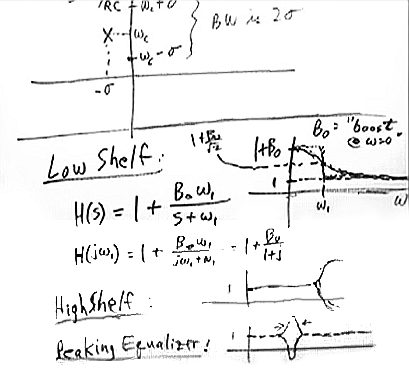
\includegraphics[scale=0.5]{frames/10a}\\
\paulhint{shot 10a taken at 4:16}\\


\subsection*{Bilinear transform}

\josquote{We are creatures of habit. Our brains are constantly trying to automate.}

$S = c \frac{1 - z^{-1}}{1 + z^{-1}}$

Usually, $c = \frac{2}{T}$ where T is the sampling interval.

% TODO: make this an itemize list?
The BLT:
\begin{itemize}
\item{preserves stability.}
\item{preserves order. }
\end{itemize}

\subsubsection*{The mapping (s-plane: left, z-plane: right)}

Critical points to map:
\begin{itemize}
\item{DC is $s = $ when $Z = 1$}
\item{dc maps to dc}
\item{$s = \inf \leftrightarrow z = -1$. infinite analogue frequency maps to
Pi, which means \textbf{No aliasing} at the price of frequency warping}
\end{itemize}

Frequency warping happens at higher frequency. Low frequency axis is in good shape.
It's only the high frequency stuff that gets compressed. As you go up
towards half the sampling rate, equal increments along the unit circle 
correspond to larger and larger increments along the omega axis. 

For some filters this is nice, like LP filters. What used to be a 6db octave is
now a hyper-accelerated rolloff. 

$\frac{1}{S}$ has a zero at infinity. That zero maps to $z = -1$. Your
point at inf maps to half the sampling rate, and you want everything to be
zero there anyways, so it's actually a good thing.

Stop bands are accelerated. If you have a guard band, you do fine. 
Sometimes it's important thatyou don't alias. If you alias a rolloff, 
the aliasing piles up, to the point where it becomes a different function.

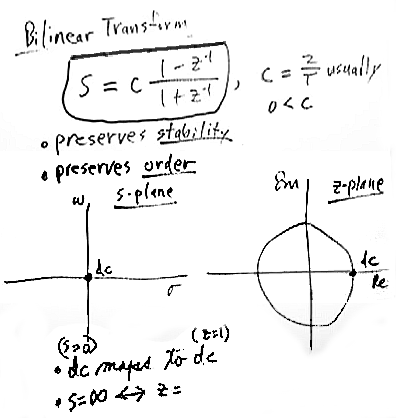
\includegraphics[scale=0.5]{frames/10b}\\
\paulhint{10b is frame taken at 9:05 or so}\\
\paulhint{10c is frame taken at 10:46 or so}

